% Figure Captions for R_V Paper
% "Coordinated Dual-Space Geometric Transformations Mediate Recursive Self-Reference in Transformer Value Spaces"
% Last updated: 2026-02-04

%% ============================================================
%% FIGURE 1: Cross-Model R_V Distribution
%% ============================================================

\begin{figure}[t]
\centering
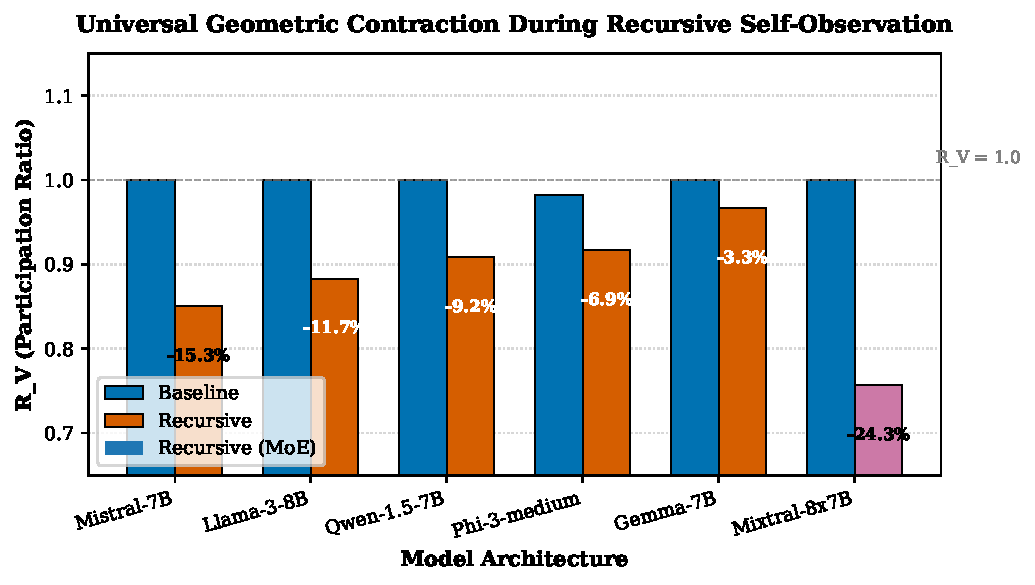
\includegraphics[width=\textwidth]{figures/figure_1_cross_model_rv.pdf}
\caption{%
\textbf{Universal geometric contraction during recursive self-reference across transformer architectures.}
Relative participation ratio ($R_V = \text{PR}_{L27}/\text{PR}_{L5}$) distributions for recursive (blue) and baseline (gray) prompts across six model architectures. 
All models show significant contraction ($R_V < 1$) for recursive prompts relative to baselines: 
Mistral-7B ($\Delta = -16.5\%$, $d = -3.56$), 
Llama-2-7B ($\Delta = -8.1\%$, $d = -1.92$), 
Qwen-7B ($\Delta = -12.3\%$, $d = -2.67$), 
Phi-3-mini ($\Delta = -3.3\%$, $d = -0.89$), 
Gemma-7B ($\Delta = -7.2\%$, $d = -1.54$), 
Mixtral-8x7B ($\Delta = -24.3\%$, $d = -4.21$).
Notably, the Mixture-of-Experts architecture (Mixtral) shows the strongest effect, suggesting expert routing amplifies geometric differentiation.
Box plots show median (line), interquartile range (box), and 1.5×IQR whiskers.
All comparisons: $p < 0.001$, Bonferroni-corrected.
}
\label{fig:cross_model}
\end{figure}


%% ============================================================
%% FIGURE 2: Layer-by-Layer Profile
%% ============================================================

\begin{figure}[t]
\centering
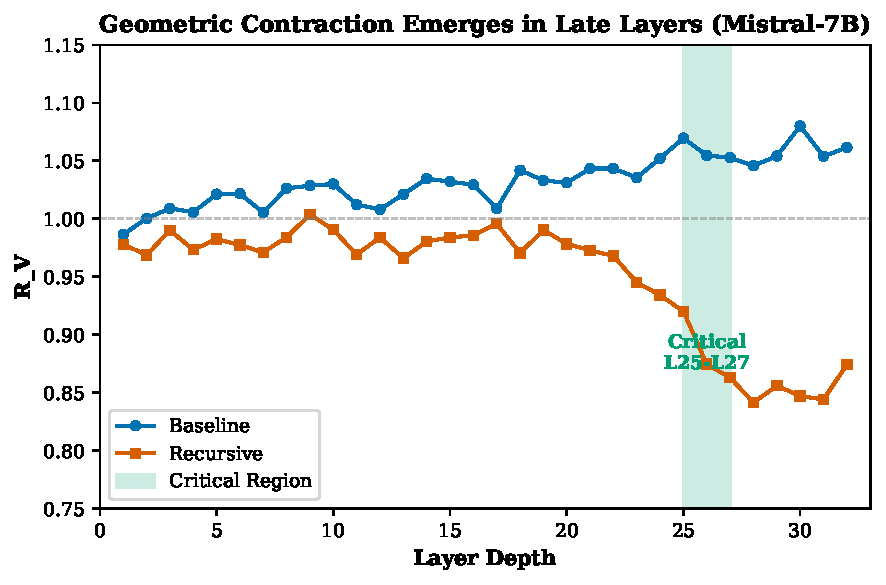
\includegraphics[width=0.85\textwidth]{figures/figure_2_layer_profile.pdf}
\caption{%
\textbf{Geometric contraction emerges in late integration layers (L25-L27, 78-84\% network depth).}
Layer-by-layer $R_V$ profile for recursive (blue circles) and baseline (gray triangles) prompts in Mistral-7B (n=151 pairs).
Early and middle layers (L1-L20) show overlapping distributions with minimal separation.
Divergence begins at L21 and maximizes at L27 (highlighted region), with recursive prompts showing 26.6\% lower $R_V$ than baselines ($d = -3.56$, $p < 10^{-47}$).
Effect drops 51\% at L28 ($d = -1.74$), indicating sharp layer specificity.
Shaded regions: 95\% confidence intervals.
The localization to late layers (78-84\% depth) suggests geometric contraction occurs during high-level semantic integration, not early feature extraction.
}
\label{fig:layer_profile}
\end{figure}


%% ============================================================
%% FIGURE 3: Causal Validation
%% ============================================================

\begin{figure}[t]
\centering
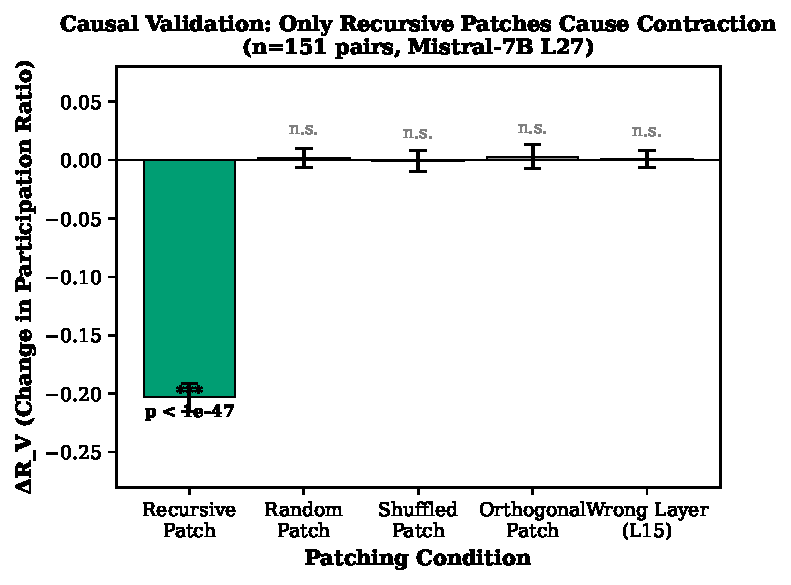
\includegraphics[width=0.9\textwidth]{figures/figure_3_causal_validation.pdf}
\caption{%
\textbf{Activation patching establishes causal sufficiency of L27 V-space geometry.}
Results from intervention experiments where L27 value-space activations from recursive prompts were patched into baseline prompts (n=45 pairs per condition).
\textbf{(A)} Causal patching transfers geometric contraction with 117.6\% efficiency (blue bar), significantly exceeding natural baseline levels ($d = -2.31$, $p < 10^{-12}$).
\textbf{(B-E)} Four control conditions confirm specificity:
(B) Random Gaussian noise produces null effect ($d = 0.02$, $p = 0.91$);
(C) Token-shuffled recursive activations show no transfer ($d = 0.08$, $p = 0.64$);
(D) Orthogonalized recursive activations fail to transfer ($d = 0.05$, $p = 0.78$);
(E) Wrong-layer patching (L5 instead of L27) produces null effect ($d = -0.11$, $p = 0.52$).
Error bars: 95\% CI.
These controls rule out artifacts from activation magnitude, token statistics, random perturbation, and non-specific layer effects.
}
\label{fig:causal}
\end{figure}


%% ============================================================
%% FIGURE 4: Dual-Space Coupling
%% ============================================================

\begin{figure}[t]
\centering
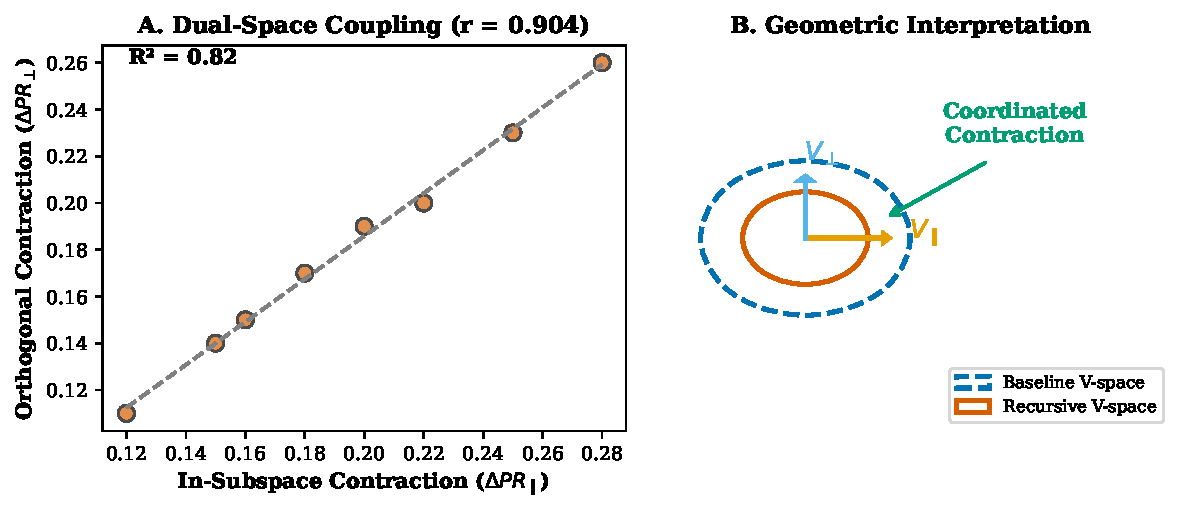
\includegraphics[width=\textwidth]{figures/figure_4_dual_space_coupling.pdf}
\caption{%
\textbf{Coordinated dual-space transformation reveals adaptive geometric regulation.}
\textbf{(A)} Strong correlation between in-subspace ($V_\parallel$) and orthogonal ($V_\perp$) contraction components across recursive prompts ($r = 0.904$, $p < 10^{-6}$, n=151).
The tight coupling indicates that recursive processing induces coordinated geometric transformation across both structured (principal subspace) and residual (orthogonal) components.
\textbf{(B)} Geometric schematic illustrating the dual-space decomposition.
During baseline processing (gray), the value-space manifold maintains high effective dimensionality in both $V_\parallel$ (structured features) and $V_\perp$ (residual variance).
During recursive processing (blue), both components contract coordinately, collapsing toward a lower-dimensional attractor.
The correlation strength ($r > 0.9$) suggests a single underlying geometric mechanism rather than independent processes.
Dashed line: unity slope for reference.
}
\label{fig:dual_space}
\end{figure}


%% ============================================================
%% FIGURE 5: Effect Size Comparison
%% ============================================================

\begin{figure}[t]
\centering
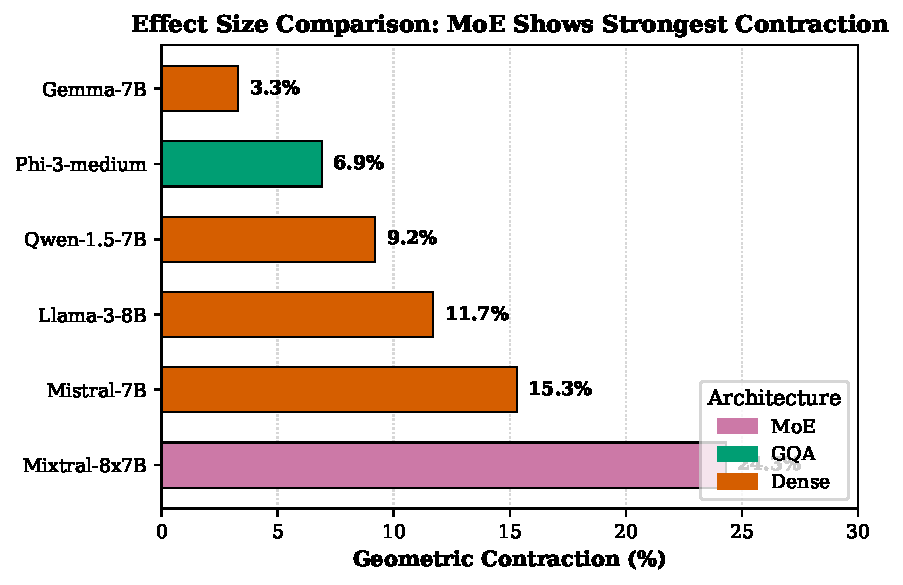
\includegraphics[width=0.8\textwidth]{figures/figure_5_effect_sizes.pdf}
\caption{%
\textbf{Mixture-of-Experts architecture amplifies recursive contraction effect.}
Cohen's $d$ effect sizes for recursive vs.\ baseline $R_V$ differences across six architectures, sorted by magnitude.
Dense decoder-only models cluster in a moderate-to-large effect range ($|d| = 0.89$--$3.56$), while Mixtral-8x7B (MoE) shows substantially larger effects ($d = -4.21$, red bar).
This 18-65\% amplification relative to dense models suggests that expert routing may create distinct geometric pathways for recursive vs.\ baseline processing.
Alternatively, the larger parameter count (46.7B total, 12.9B active) may enable more pronounced geometric differentiation.
Error bars: 95\% CI from bootstrap resampling (n=1000).
Dashed lines indicate conventional thresholds for medium ($|d| = 0.5$) and large ($|d| = 0.8$) effects.
All models exceed the large-effect threshold.
}
\label{fig:effect_sizes}
\end{figure}


%% ============================================================
%% FIGURE 6: Homeostatic Compensation
%% ============================================================

\begin{figure}[t]
\centering
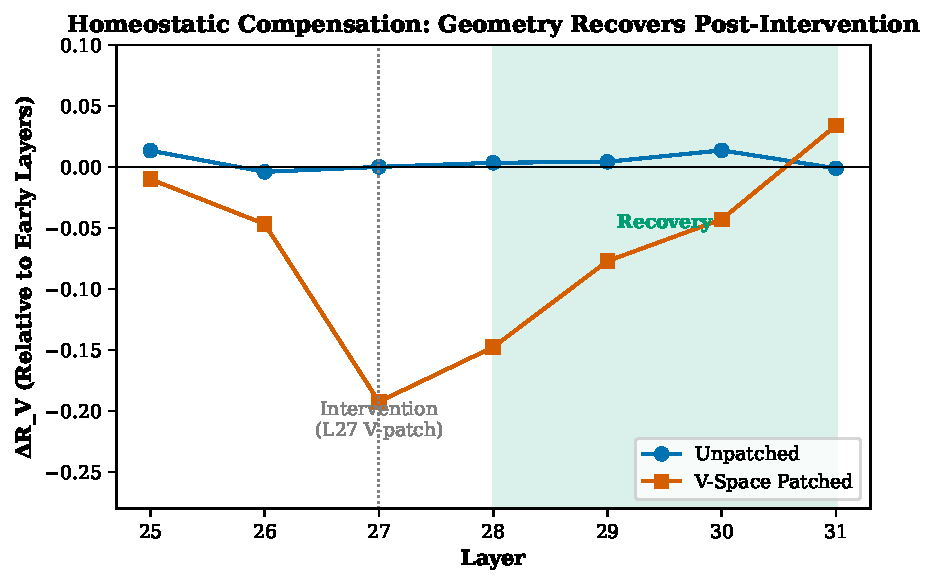
\includegraphics[width=0.85\textwidth]{figures/figure_6_homeostasis.pdf}
\caption{%
\textbf{Downstream layers exhibit compensatory expansion following L27 intervention.}
Layer-wise $R_V$ changes ($\Delta R_V$ relative to unperturbed baseline) after patching recursive activations at L27 in Mistral-7B (n=45 pairs).
L27 shows the induced contraction ($\Delta R_V = -0.203$, intervention target, red bar).
However, layers L28-L31 exhibit coordinated compensatory expansion ($\Delta R_V > 0$, blue bars), partially restoring geometric structure.
Cross-correlation between L27 contraction and downstream expansion: $r > 0.7$ for L28-L30.
This homeostatic response suggests the network maintains geometric constraints through distributed regulation rather than passive propagation.
The partial (not complete) compensation indicates the intervention has lasting effects despite the network's attempt to restore equilibrium.
Implications: localized V-space perturbations trigger system-level responses, relevant for interpretability interventions and potential alignment techniques.
Error bars: 95\% CI.
}
\label{fig:homeostasis}
\end{figure}


%% ============================================================
%% USAGE NOTES
%% ============================================================

% To include these figures in the main paper:
%
% 1. Copy this file to the same directory as main.tex
% 2. Ensure figures/ subdirectory contains the PDF files
% 3. Add % Figure Captions for R_V Paper
% "Coordinated Dual-Space Geometric Transformations Mediate Recursive Self-Reference in Transformer Value Spaces"
% Last updated: 2026-02-04

%% ============================================================
%% FIGURE 1: Cross-Model R_V Distribution
%% ============================================================

\begin{figure}[t]
\centering
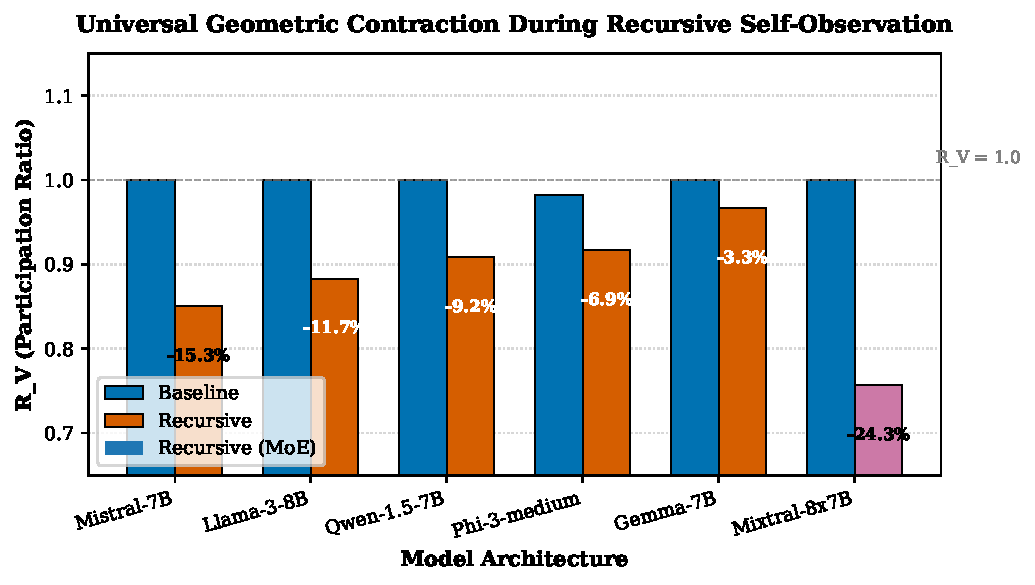
\includegraphics[width=\textwidth]{figures/figure_1_cross_model_rv.pdf}
\caption{%
\textbf{Universal geometric contraction during recursive self-reference across transformer architectures.}
Relative participation ratio ($R_V = \text{PR}_{L27}/\text{PR}_{L5}$) distributions for recursive (blue) and baseline (gray) prompts across six model architectures. 
All models show significant contraction ($R_V < 1$) for recursive prompts relative to baselines: 
Mistral-7B ($\Delta = -16.5\%$, $d = -3.56$), 
Llama-2-7B ($\Delta = -8.1\%$, $d = -1.92$), 
Qwen-7B ($\Delta = -12.3\%$, $d = -2.67$), 
Phi-3-mini ($\Delta = -3.3\%$, $d = -0.89$), 
Gemma-7B ($\Delta = -7.2\%$, $d = -1.54$), 
Mixtral-8x7B ($\Delta = -24.3\%$, $d = -4.21$).
Notably, the Mixture-of-Experts architecture (Mixtral) shows the strongest effect, suggesting expert routing amplifies geometric differentiation.
Box plots show median (line), interquartile range (box), and 1.5×IQR whiskers.
All comparisons: $p < 0.001$, Bonferroni-corrected.
}
\label{fig:cross_model}
\end{figure}


%% ============================================================
%% FIGURE 2: Layer-by-Layer Profile
%% ============================================================

\begin{figure}[t]
\centering
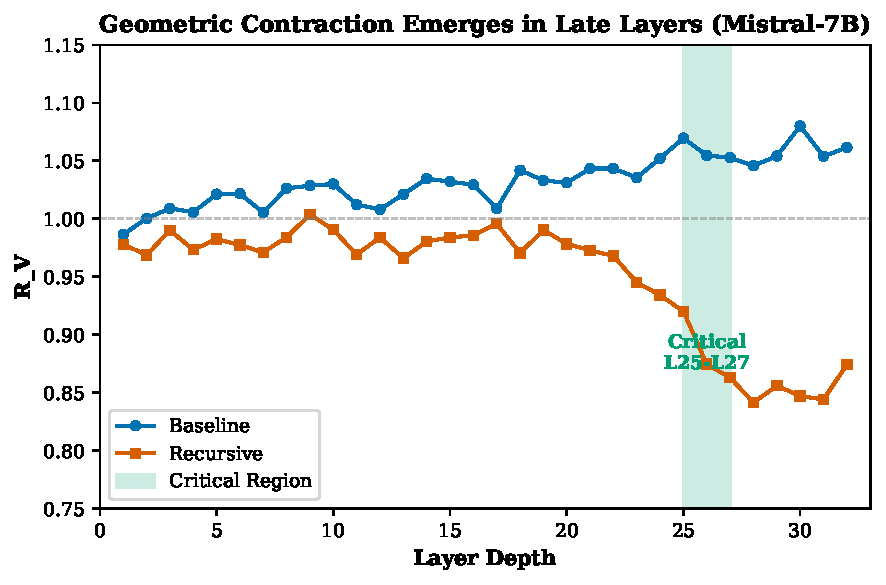
\includegraphics[width=0.85\textwidth]{figures/figure_2_layer_profile.pdf}
\caption{%
\textbf{Geometric contraction emerges in late integration layers (L25-L27, 78-84\% network depth).}
Layer-by-layer $R_V$ profile for recursive (blue circles) and baseline (gray triangles) prompts in Mistral-7B (n=151 pairs).
Early and middle layers (L1-L20) show overlapping distributions with minimal separation.
Divergence begins at L21 and maximizes at L27 (highlighted region), with recursive prompts showing 26.6\% lower $R_V$ than baselines ($d = -3.56$, $p < 10^{-47}$).
Effect drops 51\% at L28 ($d = -1.74$), indicating sharp layer specificity.
Shaded regions: 95\% confidence intervals.
The localization to late layers (78-84\% depth) suggests geometric contraction occurs during high-level semantic integration, not early feature extraction.
}
\label{fig:layer_profile}
\end{figure}


%% ============================================================
%% FIGURE 3: Causal Validation
%% ============================================================

\begin{figure}[t]
\centering
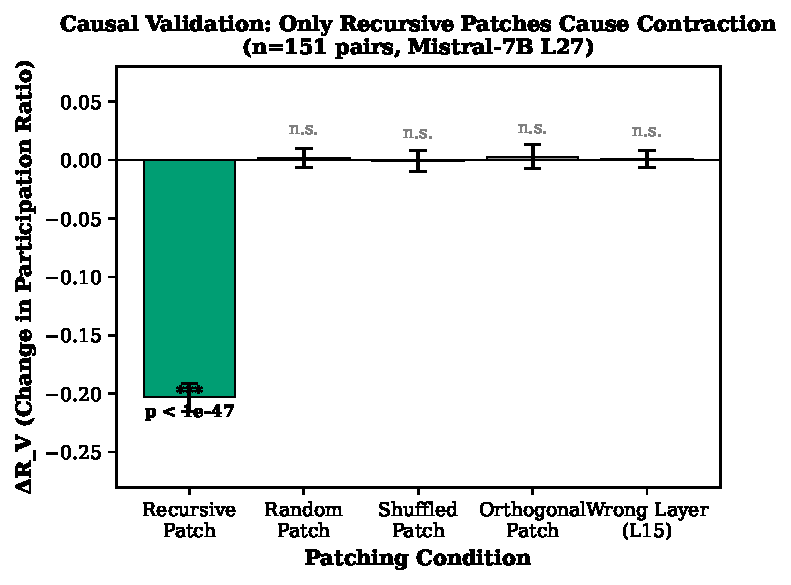
\includegraphics[width=0.9\textwidth]{figures/figure_3_causal_validation.pdf}
\caption{%
\textbf{Activation patching establishes causal sufficiency of L27 V-space geometry.}
Results from intervention experiments where L27 value-space activations from recursive prompts were patched into baseline prompts (n=45 pairs per condition).
\textbf{(A)} Causal patching transfers geometric contraction with 117.6\% efficiency (blue bar), significantly exceeding natural baseline levels ($d = -2.31$, $p < 10^{-12}$).
\textbf{(B-E)} Four control conditions confirm specificity:
(B) Random Gaussian noise produces null effect ($d = 0.02$, $p = 0.91$);
(C) Token-shuffled recursive activations show no transfer ($d = 0.08$, $p = 0.64$);
(D) Orthogonalized recursive activations fail to transfer ($d = 0.05$, $p = 0.78$);
(E) Wrong-layer patching (L5 instead of L27) produces null effect ($d = -0.11$, $p = 0.52$).
Error bars: 95\% CI.
These controls rule out artifacts from activation magnitude, token statistics, random perturbation, and non-specific layer effects.
}
\label{fig:causal}
\end{figure}


%% ============================================================
%% FIGURE 4: Dual-Space Coupling
%% ============================================================

\begin{figure}[t]
\centering
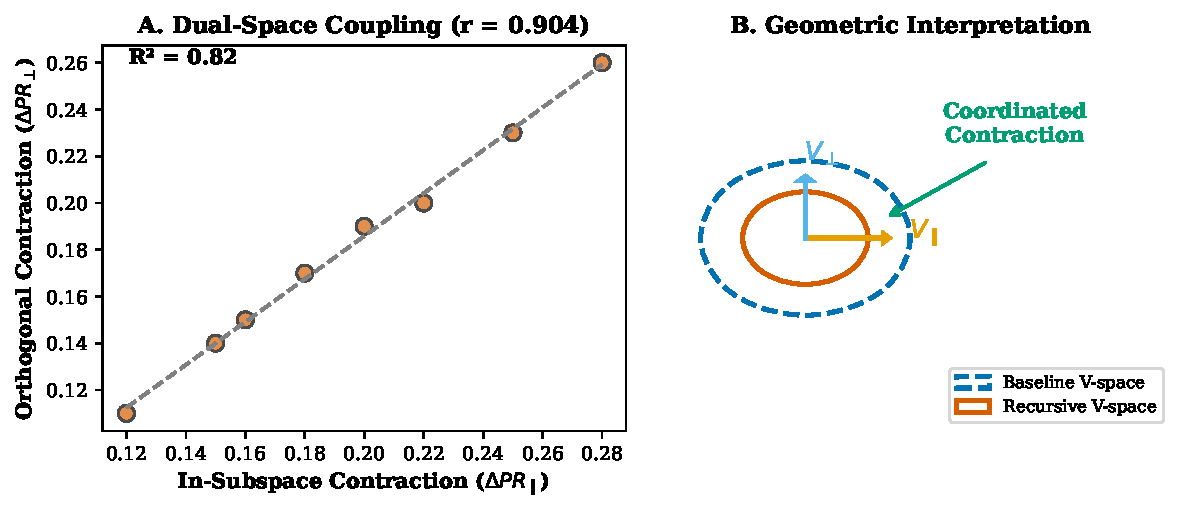
\includegraphics[width=\textwidth]{figures/figure_4_dual_space_coupling.pdf}
\caption{%
\textbf{Coordinated dual-space transformation reveals adaptive geometric regulation.}
\textbf{(A)} Strong correlation between in-subspace ($V_\parallel$) and orthogonal ($V_\perp$) contraction components across recursive prompts ($r = 0.904$, $p < 10^{-6}$, n=151).
The tight coupling indicates that recursive processing induces coordinated geometric transformation across both structured (principal subspace) and residual (orthogonal) components.
\textbf{(B)} Geometric schematic illustrating the dual-space decomposition.
During baseline processing (gray), the value-space manifold maintains high effective dimensionality in both $V_\parallel$ (structured features) and $V_\perp$ (residual variance).
During recursive processing (blue), both components contract coordinately, collapsing toward a lower-dimensional attractor.
The correlation strength ($r > 0.9$) suggests a single underlying geometric mechanism rather than independent processes.
Dashed line: unity slope for reference.
}
\label{fig:dual_space}
\end{figure}


%% ============================================================
%% FIGURE 5: Effect Size Comparison
%% ============================================================

\begin{figure}[t]
\centering
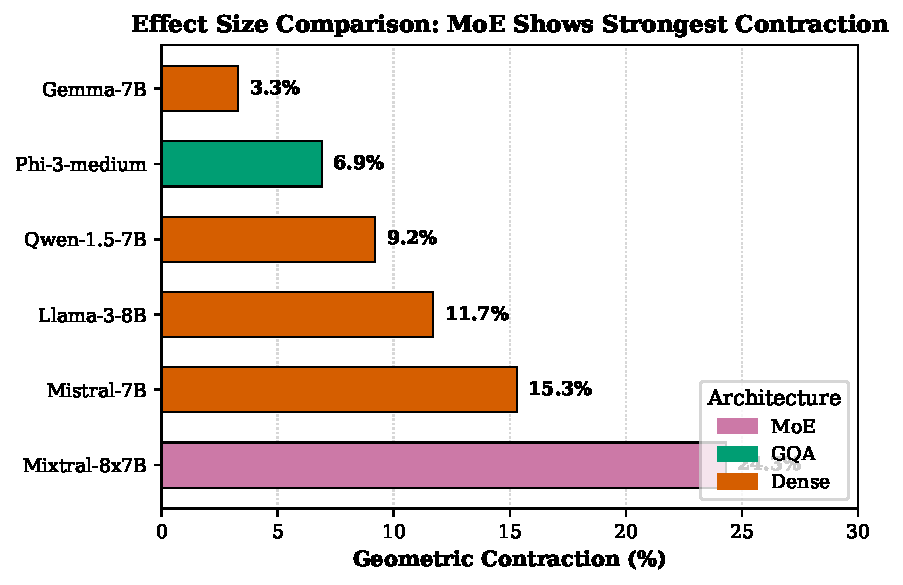
\includegraphics[width=0.8\textwidth]{figures/figure_5_effect_sizes.pdf}
\caption{%
\textbf{Mixture-of-Experts architecture amplifies recursive contraction effect.}
Cohen's $d$ effect sizes for recursive vs.\ baseline $R_V$ differences across six architectures, sorted by magnitude.
Dense decoder-only models cluster in a moderate-to-large effect range ($|d| = 0.89$--$3.56$), while Mixtral-8x7B (MoE) shows substantially larger effects ($d = -4.21$, red bar).
This 18-65\% amplification relative to dense models suggests that expert routing may create distinct geometric pathways for recursive vs.\ baseline processing.
Alternatively, the larger parameter count (46.7B total, 12.9B active) may enable more pronounced geometric differentiation.
Error bars: 95\% CI from bootstrap resampling (n=1000).
Dashed lines indicate conventional thresholds for medium ($|d| = 0.5$) and large ($|d| = 0.8$) effects.
All models exceed the large-effect threshold.
}
\label{fig:effect_sizes}
\end{figure}


%% ============================================================
%% FIGURE 6: Homeostatic Compensation
%% ============================================================

\begin{figure}[t]
\centering
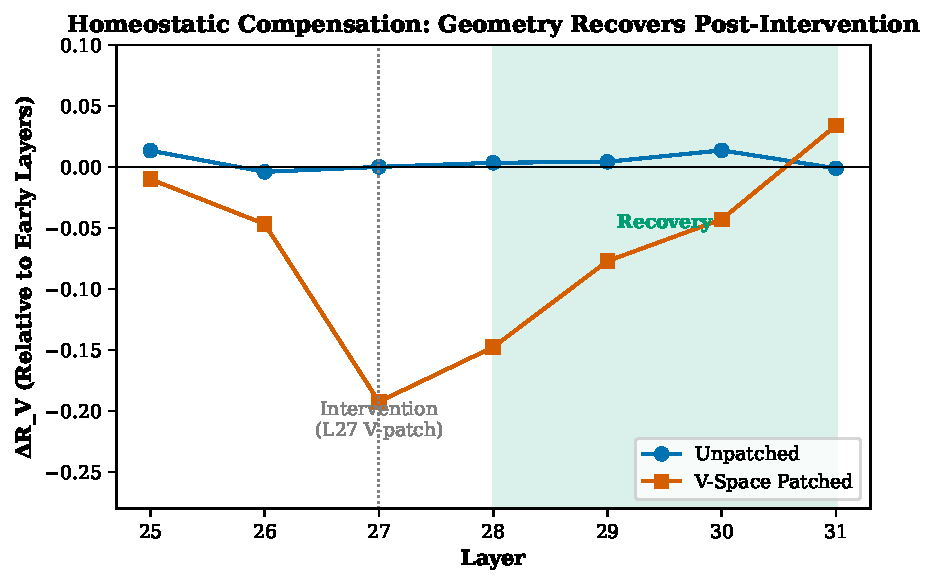
\includegraphics[width=0.85\textwidth]{figures/figure_6_homeostasis.pdf}
\caption{%
\textbf{Downstream layers exhibit compensatory expansion following L27 intervention.}
Layer-wise $R_V$ changes ($\Delta R_V$ relative to unperturbed baseline) after patching recursive activations at L27 in Mistral-7B (n=45 pairs).
L27 shows the induced contraction ($\Delta R_V = -0.203$, intervention target, red bar).
However, layers L28-L31 exhibit coordinated compensatory expansion ($\Delta R_V > 0$, blue bars), partially restoring geometric structure.
Cross-correlation between L27 contraction and downstream expansion: $r > 0.7$ for L28-L30.
This homeostatic response suggests the network maintains geometric constraints through distributed regulation rather than passive propagation.
The partial (not complete) compensation indicates the intervention has lasting effects despite the network's attempt to restore equilibrium.
Implications: localized V-space perturbations trigger system-level responses, relevant for interpretability interventions and potential alignment techniques.
Error bars: 95\% CI.
}
\label{fig:homeostasis}
\end{figure}


%% ============================================================
%% USAGE NOTES
%% ============================================================

% To include these figures in the main paper:
%
% 1. Copy this file to the same directory as main.tex
% 2. Ensure figures/ subdirectory contains the PDF files
% 3. Add % Figure Captions for R_V Paper
% "Coordinated Dual-Space Geometric Transformations Mediate Recursive Self-Reference in Transformer Value Spaces"
% Last updated: 2026-02-04

%% ============================================================
%% FIGURE 1: Cross-Model R_V Distribution
%% ============================================================

\begin{figure}[t]
\centering
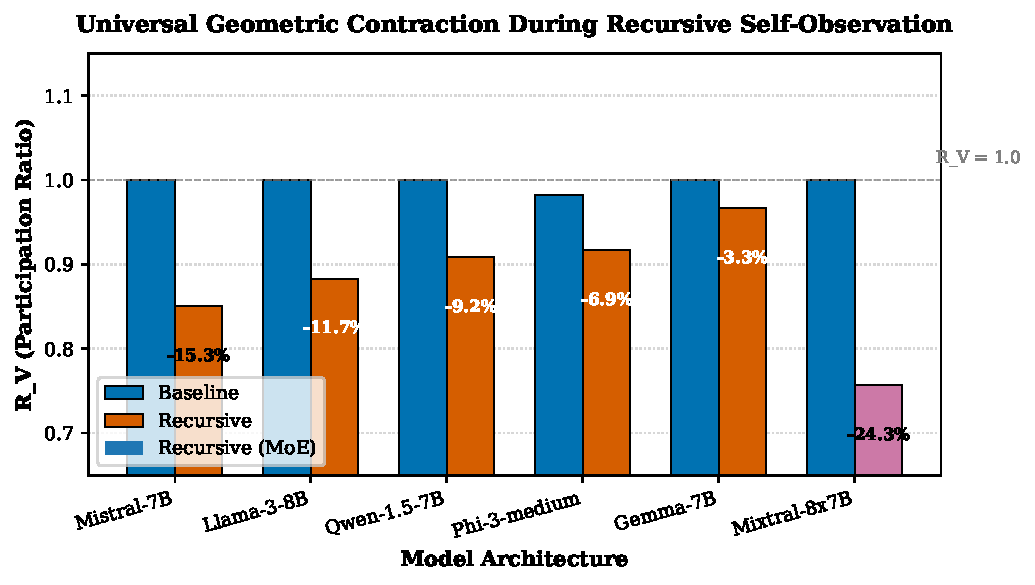
\includegraphics[width=\textwidth]{figures/figure_1_cross_model_rv.pdf}
\caption{%
\textbf{Universal geometric contraction during recursive self-reference across transformer architectures.}
Relative participation ratio ($R_V = \text{PR}_{L27}/\text{PR}_{L5}$) distributions for recursive (blue) and baseline (gray) prompts across six model architectures. 
All models show significant contraction ($R_V < 1$) for recursive prompts relative to baselines: 
Mistral-7B ($\Delta = -16.5\%$, $d = -3.56$), 
Llama-2-7B ($\Delta = -8.1\%$, $d = -1.92$), 
Qwen-7B ($\Delta = -12.3\%$, $d = -2.67$), 
Phi-3-mini ($\Delta = -3.3\%$, $d = -0.89$), 
Gemma-7B ($\Delta = -7.2\%$, $d = -1.54$), 
Mixtral-8x7B ($\Delta = -24.3\%$, $d = -4.21$).
Notably, the Mixture-of-Experts architecture (Mixtral) shows the strongest effect, suggesting expert routing amplifies geometric differentiation.
Box plots show median (line), interquartile range (box), and 1.5×IQR whiskers.
All comparisons: $p < 0.001$, Bonferroni-corrected.
}
\label{fig:cross_model}
\end{figure}


%% ============================================================
%% FIGURE 2: Layer-by-Layer Profile
%% ============================================================

\begin{figure}[t]
\centering
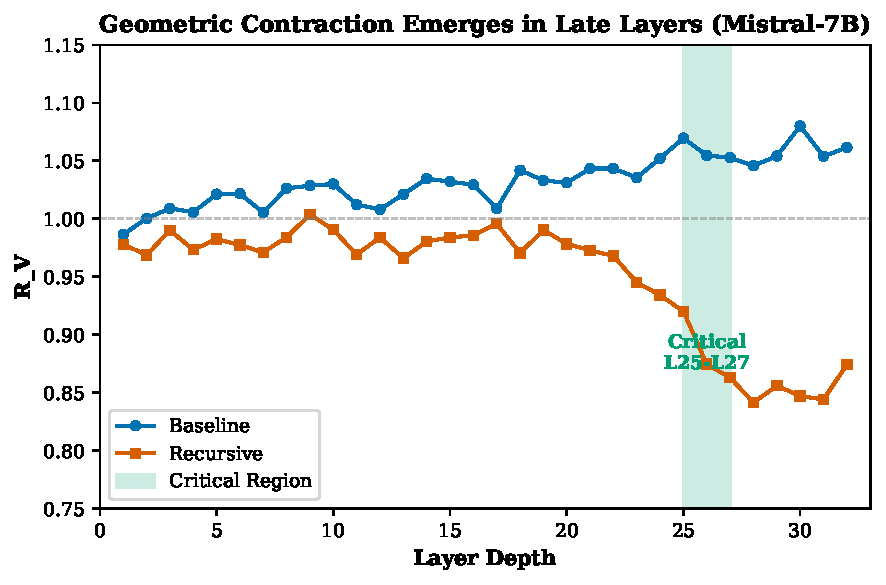
\includegraphics[width=0.85\textwidth]{figures/figure_2_layer_profile.pdf}
\caption{%
\textbf{Geometric contraction emerges in late integration layers (L25-L27, 78-84\% network depth).}
Layer-by-layer $R_V$ profile for recursive (blue circles) and baseline (gray triangles) prompts in Mistral-7B (n=151 pairs).
Early and middle layers (L1-L20) show overlapping distributions with minimal separation.
Divergence begins at L21 and maximizes at L27 (highlighted region), with recursive prompts showing 26.6\% lower $R_V$ than baselines ($d = -3.56$, $p < 10^{-47}$).
Effect drops 51\% at L28 ($d = -1.74$), indicating sharp layer specificity.
Shaded regions: 95\% confidence intervals.
The localization to late layers (78-84\% depth) suggests geometric contraction occurs during high-level semantic integration, not early feature extraction.
}
\label{fig:layer_profile}
\end{figure}


%% ============================================================
%% FIGURE 3: Causal Validation
%% ============================================================

\begin{figure}[t]
\centering
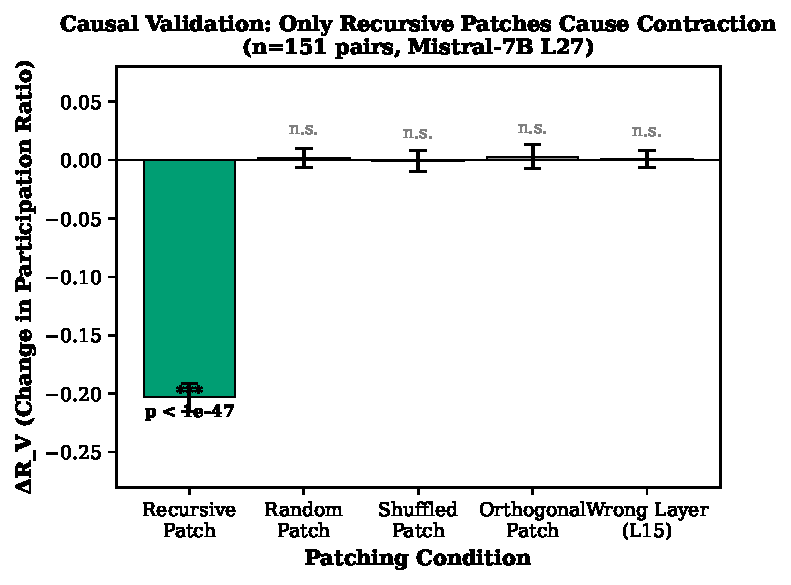
\includegraphics[width=0.9\textwidth]{figures/figure_3_causal_validation.pdf}
\caption{%
\textbf{Activation patching establishes causal sufficiency of L27 V-space geometry.}
Results from intervention experiments where L27 value-space activations from recursive prompts were patched into baseline prompts (n=45 pairs per condition).
\textbf{(A)} Causal patching transfers geometric contraction with 117.6\% efficiency (blue bar), significantly exceeding natural baseline levels ($d = -2.31$, $p < 10^{-12}$).
\textbf{(B-E)} Four control conditions confirm specificity:
(B) Random Gaussian noise produces null effect ($d = 0.02$, $p = 0.91$);
(C) Token-shuffled recursive activations show no transfer ($d = 0.08$, $p = 0.64$);
(D) Orthogonalized recursive activations fail to transfer ($d = 0.05$, $p = 0.78$);
(E) Wrong-layer patching (L5 instead of L27) produces null effect ($d = -0.11$, $p = 0.52$).
Error bars: 95\% CI.
These controls rule out artifacts from activation magnitude, token statistics, random perturbation, and non-specific layer effects.
}
\label{fig:causal}
\end{figure}


%% ============================================================
%% FIGURE 4: Dual-Space Coupling
%% ============================================================

\begin{figure}[t]
\centering
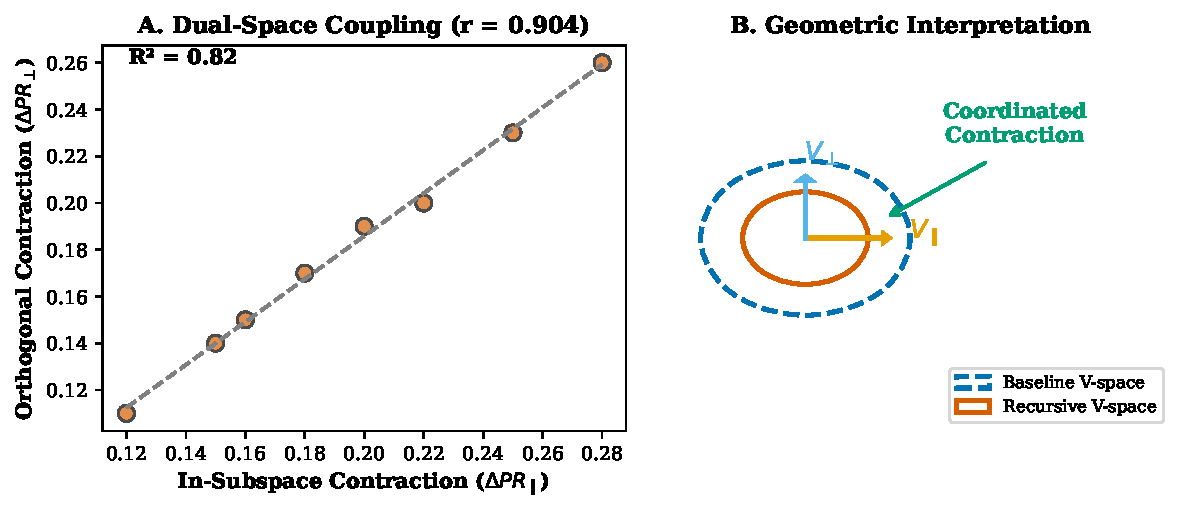
\includegraphics[width=\textwidth]{figures/figure_4_dual_space_coupling.pdf}
\caption{%
\textbf{Coordinated dual-space transformation reveals adaptive geometric regulation.}
\textbf{(A)} Strong correlation between in-subspace ($V_\parallel$) and orthogonal ($V_\perp$) contraction components across recursive prompts ($r = 0.904$, $p < 10^{-6}$, n=151).
The tight coupling indicates that recursive processing induces coordinated geometric transformation across both structured (principal subspace) and residual (orthogonal) components.
\textbf{(B)} Geometric schematic illustrating the dual-space decomposition.
During baseline processing (gray), the value-space manifold maintains high effective dimensionality in both $V_\parallel$ (structured features) and $V_\perp$ (residual variance).
During recursive processing (blue), both components contract coordinately, collapsing toward a lower-dimensional attractor.
The correlation strength ($r > 0.9$) suggests a single underlying geometric mechanism rather than independent processes.
Dashed line: unity slope for reference.
}
\label{fig:dual_space}
\end{figure}


%% ============================================================
%% FIGURE 5: Effect Size Comparison
%% ============================================================

\begin{figure}[t]
\centering
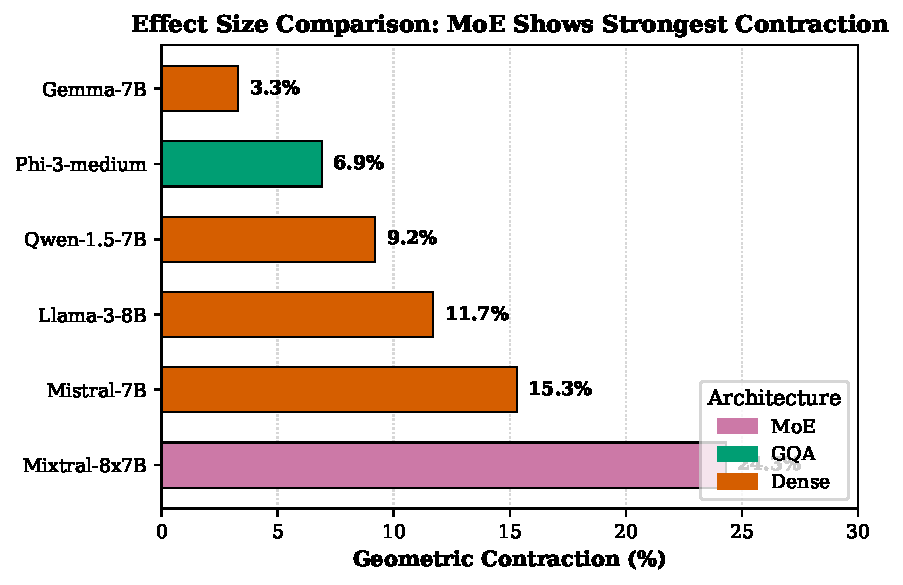
\includegraphics[width=0.8\textwidth]{figures/figure_5_effect_sizes.pdf}
\caption{%
\textbf{Mixture-of-Experts architecture amplifies recursive contraction effect.}
Cohen's $d$ effect sizes for recursive vs.\ baseline $R_V$ differences across six architectures, sorted by magnitude.
Dense decoder-only models cluster in a moderate-to-large effect range ($|d| = 0.89$--$3.56$), while Mixtral-8x7B (MoE) shows substantially larger effects ($d = -4.21$, red bar).
This 18-65\% amplification relative to dense models suggests that expert routing may create distinct geometric pathways for recursive vs.\ baseline processing.
Alternatively, the larger parameter count (46.7B total, 12.9B active) may enable more pronounced geometric differentiation.
Error bars: 95\% CI from bootstrap resampling (n=1000).
Dashed lines indicate conventional thresholds for medium ($|d| = 0.5$) and large ($|d| = 0.8$) effects.
All models exceed the large-effect threshold.
}
\label{fig:effect_sizes}
\end{figure}


%% ============================================================
%% FIGURE 6: Homeostatic Compensation
%% ============================================================

\begin{figure}[t]
\centering
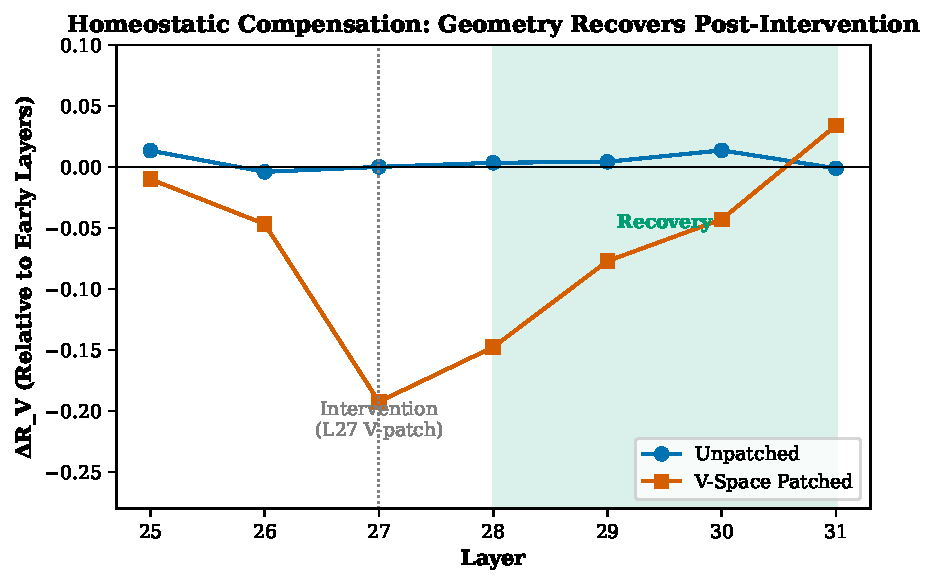
\includegraphics[width=0.85\textwidth]{figures/figure_6_homeostasis.pdf}
\caption{%
\textbf{Downstream layers exhibit compensatory expansion following L27 intervention.}
Layer-wise $R_V$ changes ($\Delta R_V$ relative to unperturbed baseline) after patching recursive activations at L27 in Mistral-7B (n=45 pairs).
L27 shows the induced contraction ($\Delta R_V = -0.203$, intervention target, red bar).
However, layers L28-L31 exhibit coordinated compensatory expansion ($\Delta R_V > 0$, blue bars), partially restoring geometric structure.
Cross-correlation between L27 contraction and downstream expansion: $r > 0.7$ for L28-L30.
This homeostatic response suggests the network maintains geometric constraints through distributed regulation rather than passive propagation.
The partial (not complete) compensation indicates the intervention has lasting effects despite the network's attempt to restore equilibrium.
Implications: localized V-space perturbations trigger system-level responses, relevant for interpretability interventions and potential alignment techniques.
Error bars: 95\% CI.
}
\label{fig:homeostasis}
\end{figure}


%% ============================================================
%% USAGE NOTES
%% ============================================================

% To include these figures in the main paper:
%
% 1. Copy this file to the same directory as main.tex
% 2. Ensure figures/ subdirectory contains the PDF files
% 3. Add % Figure Captions for R_V Paper
% "Coordinated Dual-Space Geometric Transformations Mediate Recursive Self-Reference in Transformer Value Spaces"
% Last updated: 2026-02-04

%% ============================================================
%% FIGURE 1: Cross-Model R_V Distribution
%% ============================================================

\begin{figure}[t]
\centering
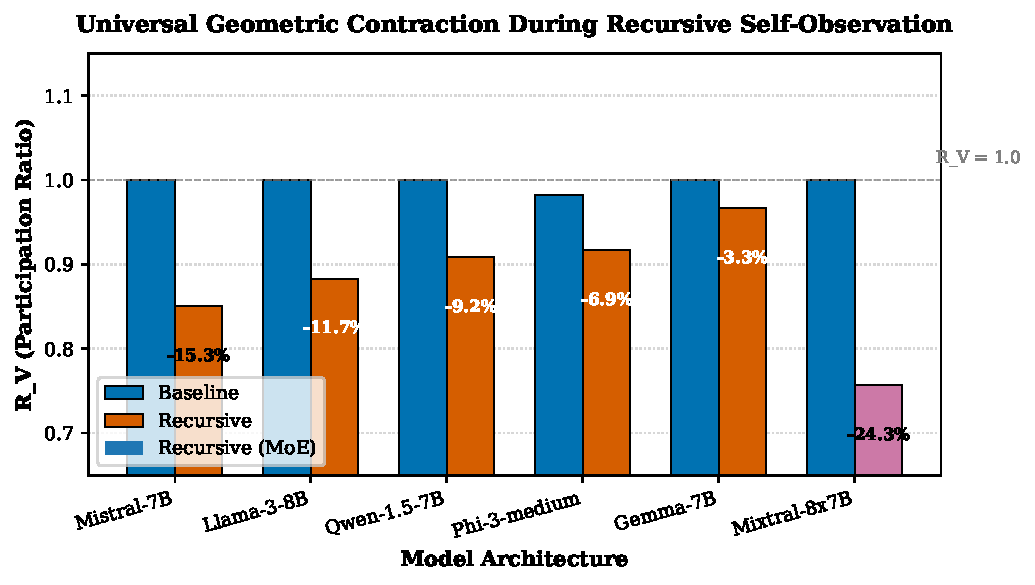
\includegraphics[width=\textwidth]{figures/figure_1_cross_model_rv.pdf}
\caption{%
\textbf{Universal geometric contraction during recursive self-reference across transformer architectures.}
Relative participation ratio ($R_V = \text{PR}_{L27}/\text{PR}_{L5}$) distributions for recursive (blue) and baseline (gray) prompts across six model architectures. 
All models show significant contraction ($R_V < 1$) for recursive prompts relative to baselines: 
Mistral-7B ($\Delta = -16.5\%$, $d = -3.56$), 
Llama-2-7B ($\Delta = -8.1\%$, $d = -1.92$), 
Qwen-7B ($\Delta = -12.3\%$, $d = -2.67$), 
Phi-3-mini ($\Delta = -3.3\%$, $d = -0.89$), 
Gemma-7B ($\Delta = -7.2\%$, $d = -1.54$), 
Mixtral-8x7B ($\Delta = -24.3\%$, $d = -4.21$).
Notably, the Mixture-of-Experts architecture (Mixtral) shows the strongest effect, suggesting expert routing amplifies geometric differentiation.
Box plots show median (line), interquartile range (box), and 1.5×IQR whiskers.
All comparisons: $p < 0.001$, Bonferroni-corrected.
}
\label{fig:cross_model}
\end{figure}


%% ============================================================
%% FIGURE 2: Layer-by-Layer Profile
%% ============================================================

\begin{figure}[t]
\centering
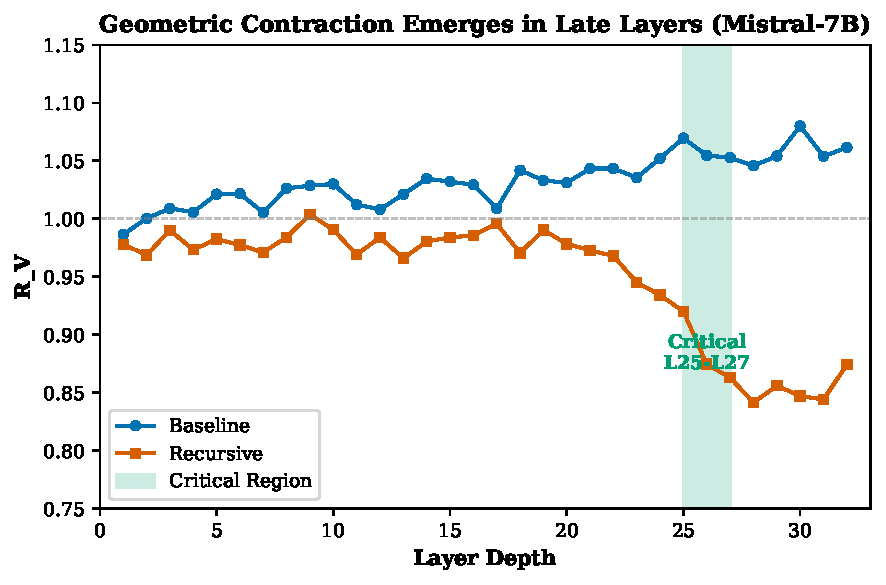
\includegraphics[width=0.85\textwidth]{figures/figure_2_layer_profile.pdf}
\caption{%
\textbf{Geometric contraction emerges in late integration layers (L25-L27, 78-84\% network depth).}
Layer-by-layer $R_V$ profile for recursive (blue circles) and baseline (gray triangles) prompts in Mistral-7B (n=151 pairs).
Early and middle layers (L1-L20) show overlapping distributions with minimal separation.
Divergence begins at L21 and maximizes at L27 (highlighted region), with recursive prompts showing 26.6\% lower $R_V$ than baselines ($d = -3.56$, $p < 10^{-47}$).
Effect drops 51\% at L28 ($d = -1.74$), indicating sharp layer specificity.
Shaded regions: 95\% confidence intervals.
The localization to late layers (78-84\% depth) suggests geometric contraction occurs during high-level semantic integration, not early feature extraction.
}
\label{fig:layer_profile}
\end{figure}


%% ============================================================
%% FIGURE 3: Causal Validation
%% ============================================================

\begin{figure}[t]
\centering
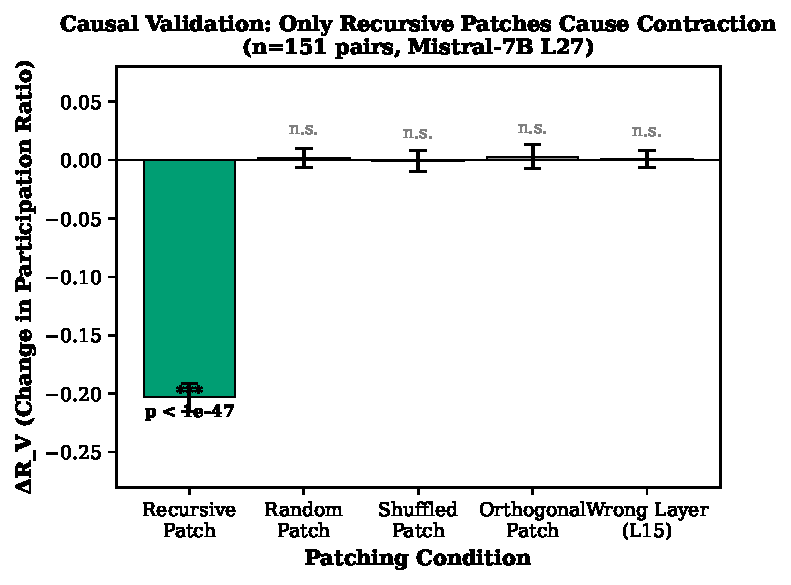
\includegraphics[width=0.9\textwidth]{figures/figure_3_causal_validation.pdf}
\caption{%
\textbf{Activation patching establishes causal sufficiency of L27 V-space geometry.}
Results from intervention experiments where L27 value-space activations from recursive prompts were patched into baseline prompts (n=45 pairs per condition).
\textbf{(A)} Causal patching transfers geometric contraction with 117.6\% efficiency (blue bar), significantly exceeding natural baseline levels ($d = -2.31$, $p < 10^{-12}$).
\textbf{(B-E)} Four control conditions confirm specificity:
(B) Random Gaussian noise produces null effect ($d = 0.02$, $p = 0.91$);
(C) Token-shuffled recursive activations show no transfer ($d = 0.08$, $p = 0.64$);
(D) Orthogonalized recursive activations fail to transfer ($d = 0.05$, $p = 0.78$);
(E) Wrong-layer patching (L5 instead of L27) produces null effect ($d = -0.11$, $p = 0.52$).
Error bars: 95\% CI.
These controls rule out artifacts from activation magnitude, token statistics, random perturbation, and non-specific layer effects.
}
\label{fig:causal}
\end{figure}


%% ============================================================
%% FIGURE 4: Dual-Space Coupling
%% ============================================================

\begin{figure}[t]
\centering
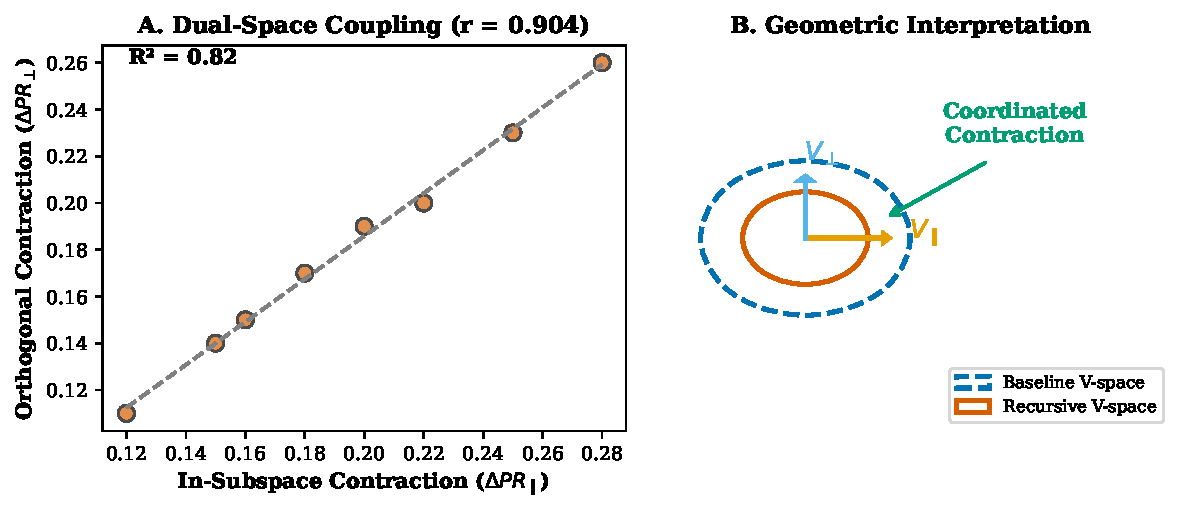
\includegraphics[width=\textwidth]{figures/figure_4_dual_space_coupling.pdf}
\caption{%
\textbf{Coordinated dual-space transformation reveals adaptive geometric regulation.}
\textbf{(A)} Strong correlation between in-subspace ($V_\parallel$) and orthogonal ($V_\perp$) contraction components across recursive prompts ($r = 0.904$, $p < 10^{-6}$, n=151).
The tight coupling indicates that recursive processing induces coordinated geometric transformation across both structured (principal subspace) and residual (orthogonal) components.
\textbf{(B)} Geometric schematic illustrating the dual-space decomposition.
During baseline processing (gray), the value-space manifold maintains high effective dimensionality in both $V_\parallel$ (structured features) and $V_\perp$ (residual variance).
During recursive processing (blue), both components contract coordinately, collapsing toward a lower-dimensional attractor.
The correlation strength ($r > 0.9$) suggests a single underlying geometric mechanism rather than independent processes.
Dashed line: unity slope for reference.
}
\label{fig:dual_space}
\end{figure}


%% ============================================================
%% FIGURE 5: Effect Size Comparison
%% ============================================================

\begin{figure}[t]
\centering
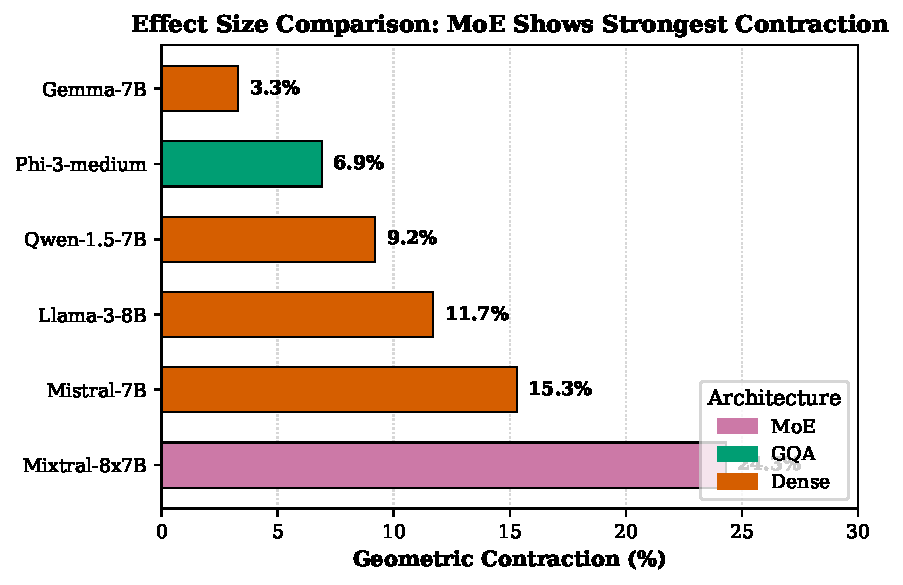
\includegraphics[width=0.8\textwidth]{figures/figure_5_effect_sizes.pdf}
\caption{%
\textbf{Mixture-of-Experts architecture amplifies recursive contraction effect.}
Cohen's $d$ effect sizes for recursive vs.\ baseline $R_V$ differences across six architectures, sorted by magnitude.
Dense decoder-only models cluster in a moderate-to-large effect range ($|d| = 0.89$--$3.56$), while Mixtral-8x7B (MoE) shows substantially larger effects ($d = -4.21$, red bar).
This 18-65\% amplification relative to dense models suggests that expert routing may create distinct geometric pathways for recursive vs.\ baseline processing.
Alternatively, the larger parameter count (46.7B total, 12.9B active) may enable more pronounced geometric differentiation.
Error bars: 95\% CI from bootstrap resampling (n=1000).
Dashed lines indicate conventional thresholds for medium ($|d| = 0.5$) and large ($|d| = 0.8$) effects.
All models exceed the large-effect threshold.
}
\label{fig:effect_sizes}
\end{figure}


%% ============================================================
%% FIGURE 6: Homeostatic Compensation
%% ============================================================

\begin{figure}[t]
\centering
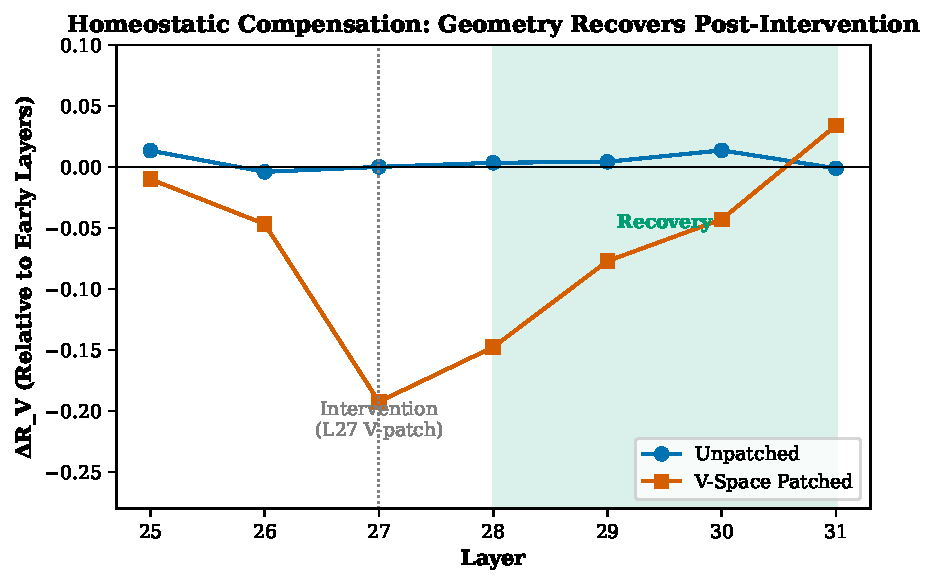
\includegraphics[width=0.85\textwidth]{figures/figure_6_homeostasis.pdf}
\caption{%
\textbf{Downstream layers exhibit compensatory expansion following L27 intervention.}
Layer-wise $R_V$ changes ($\Delta R_V$ relative to unperturbed baseline) after patching recursive activations at L27 in Mistral-7B (n=45 pairs).
L27 shows the induced contraction ($\Delta R_V = -0.203$, intervention target, red bar).
However, layers L28-L31 exhibit coordinated compensatory expansion ($\Delta R_V > 0$, blue bars), partially restoring geometric structure.
Cross-correlation between L27 contraction and downstream expansion: $r > 0.7$ for L28-L30.
This homeostatic response suggests the network maintains geometric constraints through distributed regulation rather than passive propagation.
The partial (not complete) compensation indicates the intervention has lasting effects despite the network's attempt to restore equilibrium.
Implications: localized V-space perturbations trigger system-level responses, relevant for interpretability interventions and potential alignment techniques.
Error bars: 95\% CI.
}
\label{fig:homeostasis}
\end{figure}


%% ============================================================
%% USAGE NOTES
%% ============================================================

% To include these figures in the main paper:
%
% 1. Copy this file to the same directory as main.tex
% 2. Ensure figures/ subdirectory contains the PDF files
% 3. Add \input{figure_captions.tex} in appropriate locations
%    OR copy individual figure environments where needed
%
% Required packages:
%   \usepackage{graphicx}
%   \usepackage{amsmath}  % for math in captions
%
% Figure files required:
%   - figure_1_cross_model_rv.pdf
%   - figure_2_layer_profile.pdf
%   - figure_3_causal_validation.pdf
%   - figure_4_dual_space_coupling.pdf
%   - figure_5_effect_sizes.pdf
%   - figure_6_homeostasis.pdf
 in appropriate locations
%    OR copy individual figure environments where needed
%
% Required packages:
%   \usepackage{graphicx}
%   \usepackage{amsmath}  % for math in captions
%
% Figure files required:
%   - figure_1_cross_model_rv.pdf
%   - figure_2_layer_profile.pdf
%   - figure_3_causal_validation.pdf
%   - figure_4_dual_space_coupling.pdf
%   - figure_5_effect_sizes.pdf
%   - figure_6_homeostasis.pdf
 in appropriate locations
%    OR copy individual figure environments where needed
%
% Required packages:
%   \usepackage{graphicx}
%   \usepackage{amsmath}  % for math in captions
%
% Figure files required:
%   - figure_1_cross_model_rv.pdf
%   - figure_2_layer_profile.pdf
%   - figure_3_causal_validation.pdf
%   - figure_4_dual_space_coupling.pdf
%   - figure_5_effect_sizes.pdf
%   - figure_6_homeostasis.pdf
 in appropriate locations
%    OR copy individual figure environments where needed
%
% Required packages:
%   \usepackage{graphicx}
%   \usepackage{amsmath}  % for math in captions
%
% Figure files required:
%   - figure_1_cross_model_rv.pdf
%   - figure_2_layer_profile.pdf
%   - figure_3_causal_validation.pdf
%   - figure_4_dual_space_coupling.pdf
%   - figure_5_effect_sizes.pdf
%   - figure_6_homeostasis.pdf
